%%%%%%%%%%%%%%%%%%%%%%%%%%%%%%%%%%%%%%%%%%%%%%%%%%%%%%%%%%%%%%%%%%%%%%%%%%%%%%%%
%%%%%%%%%%%%%%%%%%%%%%%%%%%%%%%%%%% PREAMBLE %%%%%%%%%%%%%%%%%%%%%%%%%%%%%%%%%%%
%%%%%%%%%%%%%%%%%%%%%%%%%%%%%%%%%%%%%%%%%%%%%%%%%%%%%%%%%%%%%%%%%%%%%%%%%%%%%%%%


%%%%%%%%%%%%%%%%%%%%%%%%%%%%%%%%%%%%%%%%%
%%%%%%%%%%%%%%%%% CLASS %%%%%%%%%%%%%%%%%
%%%%%%%%%%%%%%%%%%%%%%%%%%%%%%%%%%%%%%%%%

\documentclass[10pt,letterpaper]{article}

%%%%%%%%%%%%%%%%%%%%%%%%%%%%%%%%%%%%%%%%
%%%%%%%%%%%%%%% PACKAGES %%%%%%%%%%%%%%%
%%%%%%%%%%%%%%%%%%%%%%%%%%%%%%%%%%%%%%%%

\usepackage[debugshow, final]{graphicx}
\usepackage{amsmath, amssymb, amsthm, amsfonts}
\usepackage{enumerate}
\usepackage{staves}
\usepackage{fancybox}
\usepackage{ltablex}
\usepackage{fancyhdr}
\usepackage{setspace}
\usepackage{framed}
\usepackage[left = 1in, right=1.5in]{geometry}
\usepackage{titling}

\usepackage{natbib}
\usepackage{rotating}
\usepackage{setspace}
\usepackage{multicol}

\usepackage{pdflscape}
\usepackage{lscape}
\usepackage[table]{xcolor}

\usepackage[T1]{fontenc}
%% \usepackage{subfigure}
\usepackage{hyperref}
\usepackage{cclicenses}
\usepackage[all]{hypcap}
\usepackage{listings}
\usepackage{titlesec}

\usepackage{stix}
%%\usepackage{textcomp}

\usepackage{tocloft}
\renewcommand{\cftsecleader}{\cftdotfill{\cftdotsep}}

%%%%%%%%%%%%%%%%%%%%%%%%%%%%%%%%%%%%%%%%
%%%%%%%%%%%%%%% SETTINGS %%%%%%%%%%%%%%%
%%%%%%%%%%%%%%%%%%%%%%%%%%%%%%%%%%%%%%%%

\pagestyle{fancy}
% \lhead{}
% \chead{}
% \rhead{}
% \cfoot{\thepage}

\author{Prepared by Jonathan P.\ Olmsted}

\title{Just Another Introduction to \LaTeX{}: A (Very) Short Course}

\date{Updated: \today}

\definecolor{mygray}{rgb}{0.95,0.95,0.95}


\titleformat{\section}{\large\bf\sf\color{purple}}{\thesection\hspace{5pt}$\vert$}{5pt}{}

\pretitle{\begin{center}\huge\bf\sf\color{purple}}
  \posttitle{\par\end{center}\vspace{1cm}}

\hypersetup{
  colorlinks=true,       % false: boxed links; true: colored links
  linkcolor=blue,          % color of internal links (change box color with linkbordercolor)
  citecolor=green,        % color of links to bibliography
  filecolor=magenta,      % color of file links
  urlcolor=cyan           % color of external links
}

\lstset{ %
  backgroundcolor=\color{white},   % choose the background color; you must add \usepackage{color} or \usepackage{xcolor}
  basicstyle=\footnotesize\ttfamily,        % the size of the fonts that are used for the code
  commentstyle=\scriptsize\color{red},
  breakatwhitespace=false,         % sets if automatic breaks should only happen at whitespace
  breaklines=false,                 % sets automatic line breaking
  captionpos=b,                    % sets the caption-position to bottom
  extendedchars=true,              % lets you use non-ASCII characters; for 8-bits encodings only, does not work with UTF-8
  frame=single,                    % adds a frame around the code
  columns=fullflexible,
  keepspaces=true,                 % keeps spaces in text, useful for keeping indentation of code (possibly needs columns=flexible)
  language=tex,                 % the language of the code
  numbers=none,                    % where to put the line-numbers; possible values are (none, left, right)
  numbersep=5pt,                   % how far the line-numbers are from the code
  numberstyle=\texttt,
  showspaces=false,                % show spaces everywhere adding particular underscores; it overrides 'showstringspaces'
  showstringspaces=false,          % underline spaces within strings only
  showtabs=false,                  % show tabs within strings adding particular underscores
  stepnumber=1,                    % the step between two line-numbers. If it's 1, each line will be numbered
  showlines=false,
  %%keywordstyle=\color{blue},
  tabsize=2                       % sets default tabsize to 2 spaces
}


%%%%%%%%%%%%%%%%%%%%%%%%%%%%%%%%%%%%%%%%%
%%%%%%%%%%%%% CUSTOM MACROS %%%%%%%%%%%%%
%%%%%%%%%%%%%%%%%%%%%%%%%%%%%%%%%%%%%%%%%

\let\margin\marginpar
\newcommand\myMargin[1]{
  \margin{\singlespace\raggedright\scriptsize
    \textsf{#1}}
}
\renewcommand{\marginpar}[1]{\myMargin{#1}}

\newcommand\blurb[1]{
  \begin{center}
    \parbox[h]{.75\linewidth}{
      \footnotesize \singlespace
      #1
    }
  \end{center}
}

\newcommand{\tsl}{\textbf{\textsf{the starlab}}}


%%%%%%%%%%%%%%%%%%%%%%%%%%%%%%%%%%%%%%%%%%%%%%%%%%%%%%%%%%%%%%%%%%%%%%%%%%%%%%%
%%%%%%%%%%%%%%%%%%%%%%%%%%%%%%%%%%% CONTENT %%%%%%%%%%%%%%%%%%%%%%%%%%%%%%%%%%%
%%%%%%%%%%%%%%%%%%%%%%%%%%%%%%%%%%%%%%%%%%%%%%%%%%%%%%%%%%%%%%%%%%%%%%%%%%%%%%%

\begin{document}

\begin{titlepage}
  \maketitle
\end{titlepage}

\section*{Introduction to this Short Course}

\paragraph{Purpose.} The aim of this document is to serve as a set of guided
lessons in creating \LaTeX{} documents and to serve as an example of the kind of
documents that can be produced with the \LaTeX{} family of tools. It is not and
does not aim to be comprehensive.

\paragraph{About.} This document was originally prepared by the author during
his tenure as \tsl{} fellow for the incoming graduate student cohort in the
Political Science department at the University of Rochester. Previous versions
of the short course and the corresponding materials are available at \tsl{}'s
website (\url{http://www.rochester.edu/college/psc/thestarlab/}). This document
began as an adaptation of Arthur Spirling's version. It's current version may or
may not have diverged considerably.

In addition to the supplemental files used for the various exercises included in
this version, all files required to create this document are available at
\url{https://github.com/olmjo/LaTeX-Intro}.

\paragraph{Rights.}This document is released under the Creative
Commons Attribution license \by{}.

\paragraph{Comments.}If you have any comments, questions, or concerns regarding
this document please contact Jonathan Olmsted
\href{mailto:jpolmsted@gmail.com}{\texttt{jpolmsted@gmail.com}}.

\pagebreak

\tableofcontents

\pagebreak

\part{An Introduction to Using \LaTeX{}}

\section{What is \LaTeX{} (lay-teck) or LaTeX, but not latex or Latex?}

\begin{itemize}

\item \LaTeX{} is an open, document--preparation system used by many students,
  academics, and publishers whose content involves technical topics or complex
  structure (\textit{e.g.}\ math professors, engineers, you).

\item \LaTeX{} is a kind of markup language. This means \LaTeX{} files
  explicitly articulate both the \textit{content} and the
  \textit{structure}. Other markup languages include HTML, XML and Markdown. If
  you go to the New York Times webpage (\url{www.nytimes.com}) and view the HTML
  source for the main page it will look (incredibly) different from how that web
  page is rendered by your browser. \footnote{In the Google Chrome browser you
    can view source by navigating to the ``Tools'' menu item and choosing ``View
    Source''.} The web page is written in the HTML markup language, but then a
  separate program renders the page. The main point here is that ``creation''
  and ``consumption'' are conceptually distinct. LaTeX{} is much more similar to
  HTML source than it is to a word processor (\textit{e.g.}  MS Word, OpenOffice
  Writer, Google Documents). When you work with a \LaTeX{} file, you describe
  how the file should look, but this is not displayed for you in real-time.
\end{itemize}

\section{Why Would You Use \LaTeX{}?}

\LaTeX{} has a number of distinct advantages:

\begin{itemize}

\item A \LaTeX{} document can be very pleasing to the eye without the need for
  any customization.

\item When your focus is on producing content, but are neither a publisher nor a
  graphic designer, \LaTeX{} lets you focus on the content: \LaTeX{} separates
  content from appearance.

\item \LaTeX{}'s ability to incorporate math is un-rivaled.

% \item People in this discipline who do things like what you will do
%   will expect it.

\item You will never get locked out from the fruits of your intellectual labor
  because of licenses or old software. The software is open and the files you
  create are ``flat text'' files. If someone has a computer, they can read your
  \LaTeX{} files.

\item Also, because it relies on plain text files, collaboration among multiple
  contributors to a single project can be managed \textit{much} more readily.

\item The markup code for \LaTeX{} math is one of the canonical ways
  of representing math in plain-text environments (\textit{e.g.}\
  email, instant messaging).

\end{itemize}

\section{How Does \LaTeX{} Work?}

\par The process of creating a \LaTeX{} document is quite different from
creating one in a word processor. There is, undeniably, a learning curve.

Although most of the technical details can safely be ignored, some understanding
of the different components comprising a functioning \LaTeX{} workflow is
helpful at the outset. And, understanding how pieces fit together makes asking
for help much easier. A basic representation of the workflow is given in
Figure~\ref{fig:workflow}.

\begin{figure}
  \caption{Example \LaTeX{} Workflow}
  \label{fig:workflow}
  \begin{center}
    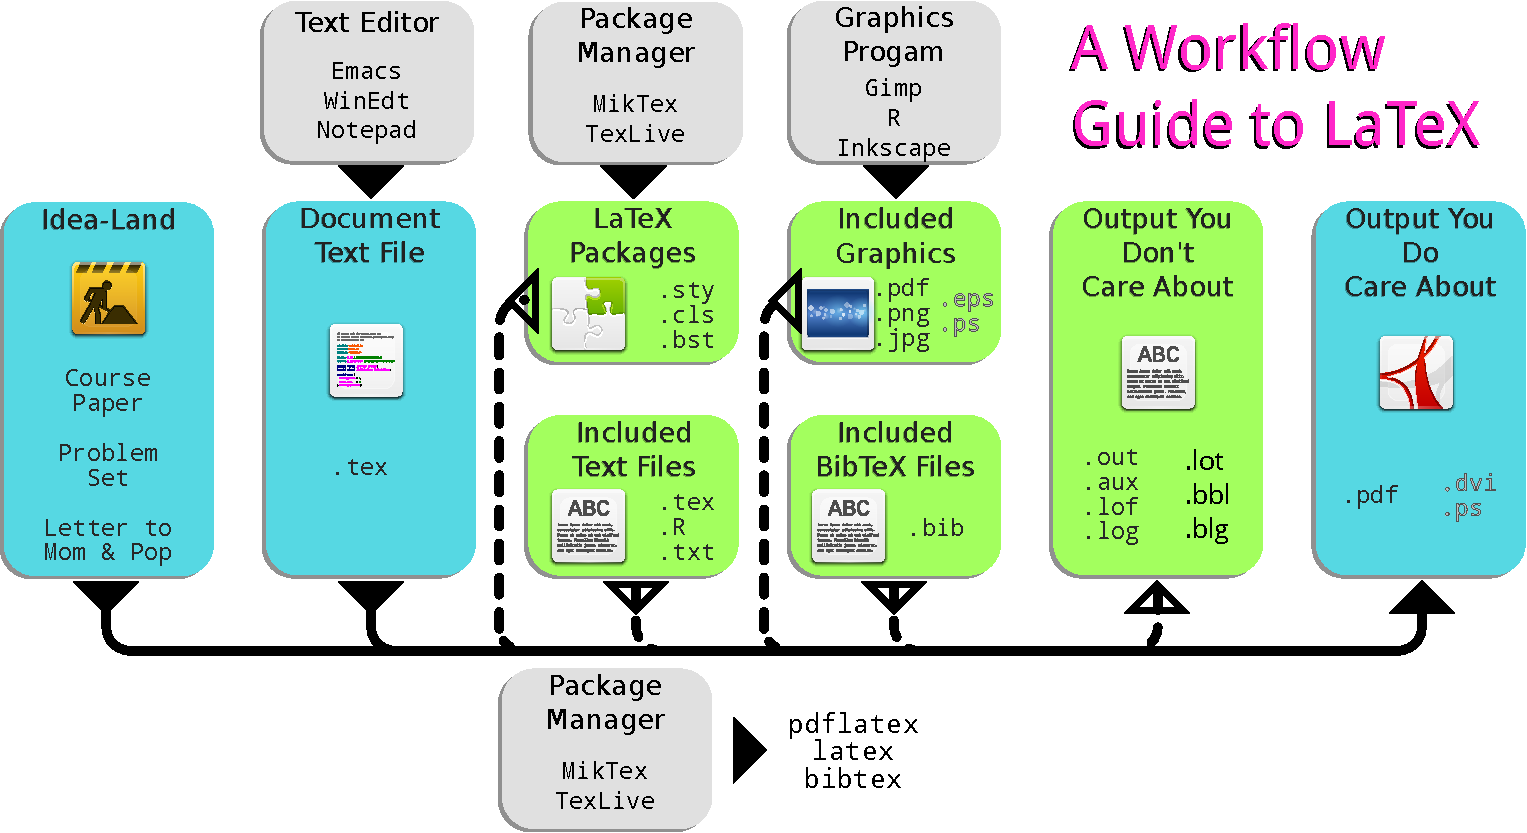
\includegraphics[scale=.5,angle=90]{extra/workflow.pdf}

    \blurb{An example workflow using \LaTeX{} to produce the output you care
      about. Blue regions represent the components you will focus on the most on
      a daily basis. Grey regions represent the software that will help you get
      from start to finish. Green regions represent intermediate or sometimes
      option files that are less focal.}
  \end{center}
\end{figure}


The basic steps to creating a document are:
\begin{enumerate}
\item Have an idea!

\item Create a plain text document containing the content in a text
  editor. These plain text files a typically given a file extension of
  \verb=.tex=.

\item Process the plain text document with the \LaTeX{} ``program''.

\item \LaTeX{} pulls in any additional files that are asked for---but they have
  to be asked for---and creates, among other files, the document you will print
  or email. Most of the time, this is a PDF file.

\item View the result/rendering of your \LaTeX{} document by opening the PDF
  file.

\item Be happy.

\end{enumerate}

Notice that this is different from the word processor workflow. In
that case, Steps 2, 4, and 5 are basically integrated. Step 3 is
unnecessary. Step 6 may or may not happen.

What now follows is some more explanation of the kind of software will be needed
for each step.

\paragraph{Step 2} You could use any number of other text editors. Many Windows
users like WinEdt or Sublime. Other options include nerdier text editors like
Emacs. It's best to find a text editor with well-documented \LaTeX{}
integration. This will facilitate the next steps after you write your file.

We typically denote \LaTeX{} files with the \texttt{.tex} file
extension. Although it isn't necessary in some cases, most software and
operating systems will make your life easier if you are willing to name \LaTeX{}
files what they expect you to name them.

\paragraph{Step 3} If you have chosen your text editor well, you can achieve
this from within that program. For example, WinEdt has a button you can just
click to process your \texttt{.tex} file.

\par Also, \LaTeX{}-ing your document can proceed through one of two different
branches. I will focus on the \texttt{pdflatex} branch and not the
\texttt{latex} branch. \texttt{pdflatex} will convert your \texttt{.tex} file
into a \texttt{.pdf} document. Included images must be \texttt{.jpg},
\texttt{.png}, \texttt{.pdf}, or \texttt{.svg} files. These inputs and PDF
output are far more common now, so that is the focus here.

\paragraph{Step 4} Sometimes markup in the \LaTeX{} file will require
contributed packages which tell the \LaTeX{} how the content should be
rendered. This is one of the critical benefits of using a system like \LaTeX{}:
you can utilize functionality that many other people have already provided
rather than re-invent it or do without.

However, making sure these packages are placed in the right spot on your system
and up-to-date can be involved and opaque to the newcomer. \LaTeX{} package
managers simplify this. On Window machines, MikTeX is often used. By and large,
you can and should ignore this fact in the beginning of your \LaTeX{}
experience. What is important is to realize the following:
\[
\textrm{\LaTeX{}} \neq \textrm{a text editor} \neq \textrm{a package manager
  (e.g., MikTeX)}.
\]

\paragraph{Step 5} Once you have a PDF file, you can view it in your preferred
PDF viewer like Adobe Reader. A well-chosen text editor will make this viewing
easy, too.

\paragraph{Step 6} No software necessary.

\section{Exercise: Your First Document}

\begin{enumerate}
\item Go to
  \url{https://github.com/olmjo/LaTeX-Intro/tree/master/Extra_Materials}.

\item Save the file \texttt{FakeFile.tex} to your desktop.

\item Open this file in your text editor.

\item Run \texttt{pdflatex} on the \texttt{.tex} file and view it.

\item Notice how many ancillary files this process creates.

\end{enumerate}

The contents of this file are as follows:

\lstinputlisting[caption=\texttt{FakeFile.tex}]{extra/FakeFile.tex}

The resultant PDF file should look like Figure~\ref{fig:output}.

\begin{figure}
  \caption{\texttt{FakeFile.pdf} Output} \label{fig:output}
  \begin{center}
    \fbox{
      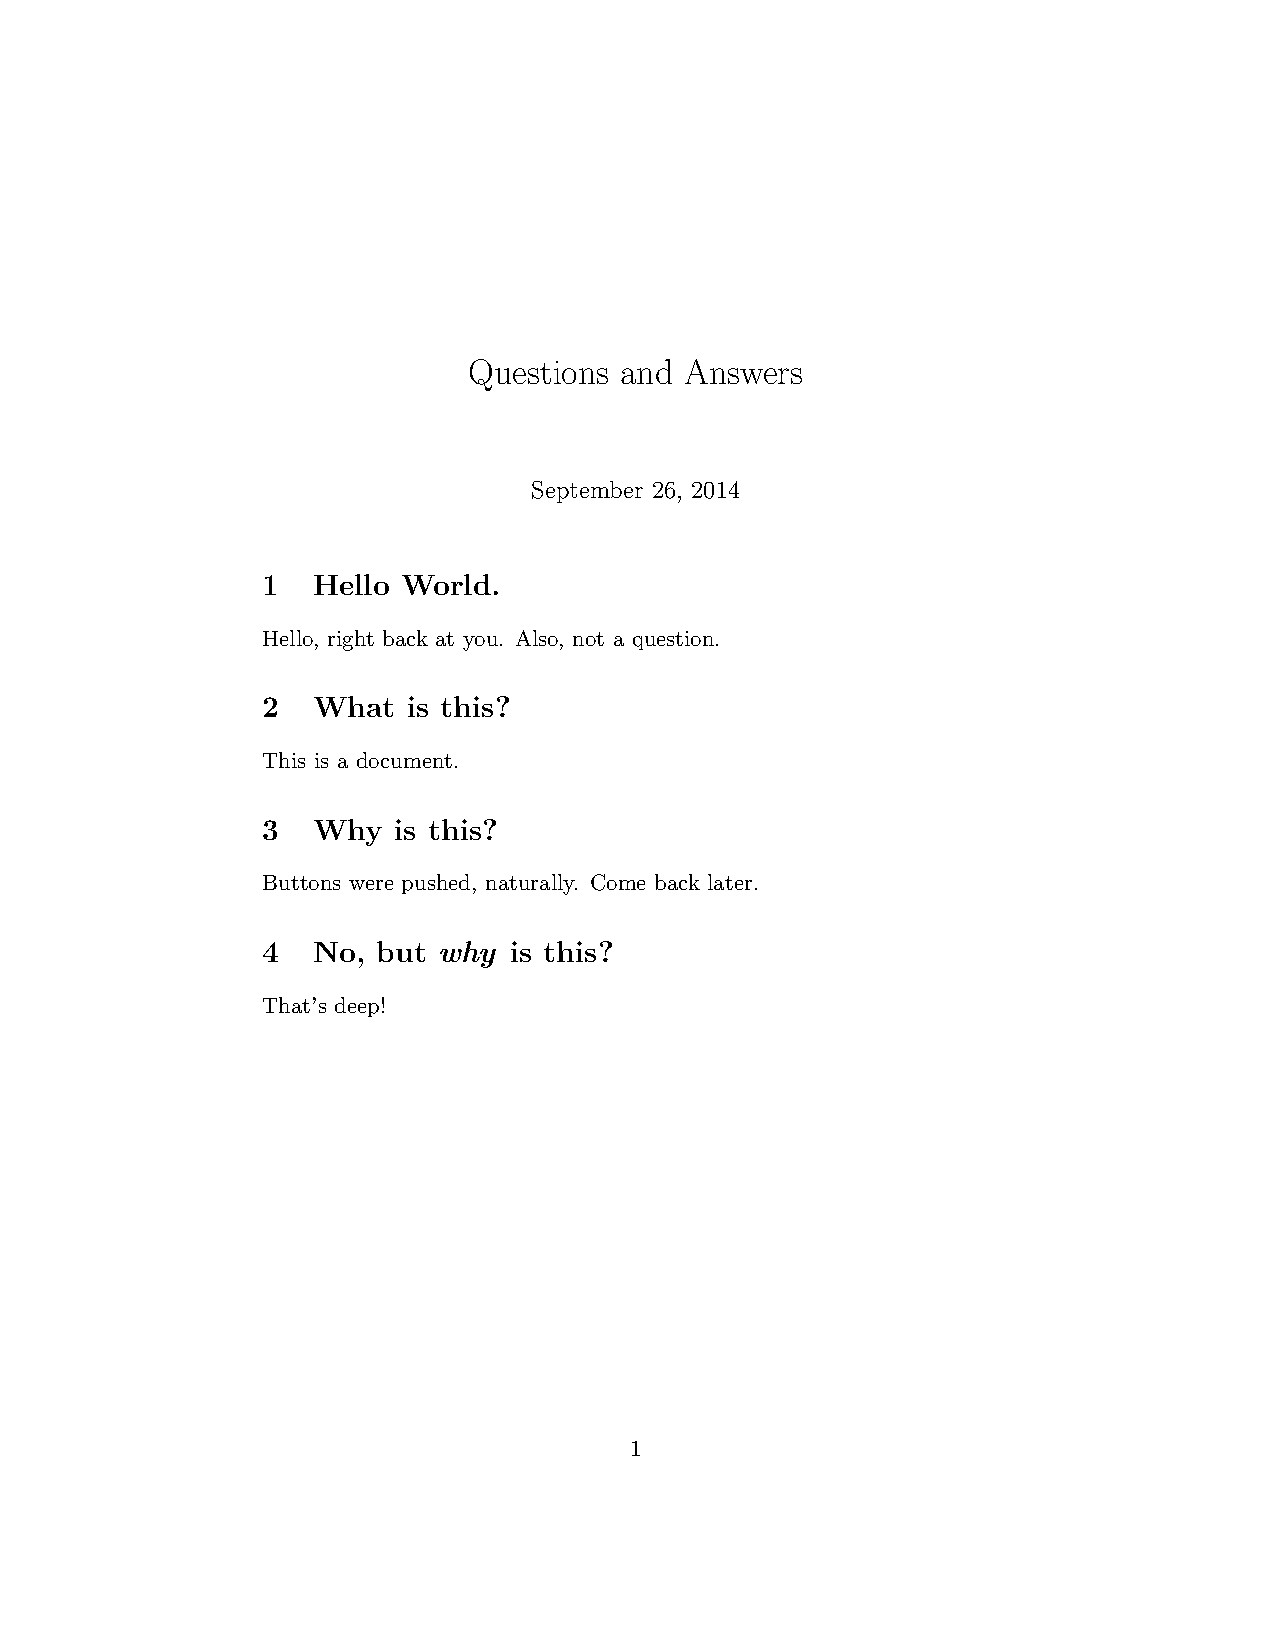
\includegraphics[scale=.5]{extra/FakeFile}
    }

    \blurb{This figure shows the PDF output created by the input \LaTeX{} file
      \texttt{FakeFile.tex}.
    }

  \end{center}
\end{figure}


You have successfully created your first \LaTeX{} document and
simultaneously learned to always keep \LaTeX{} files/projects in
separate directories because the output will create clutter.


%%% Local Variables:
%%% mode: latex
%%% TeX-master: "../../tutorial"
%%% End:


\clearpage
\pagebreak

\part{Basic Content in LaTeX{}}

\section{\LaTeX{}'s Interpretation of Plain Text}

\begin{itemize}
\item The entire \texttt{.tex} file you write will contain only characters on
  your keyboard. That means, somehow, the characters on your keyboard you need
  to represent: a, A, $\alpha$, $\mathbb{A}$, \`a, \texttt{A}, $_a$, and \"A.

\item The file that you write will be composed entirely of the characters in
  Table~\ref{tab:chars}. This is true no matter what kind of crazy symbols are
  ultimately included, such as \staveVI.

  \begin{table}[h]
    \centering
    \begin{center}
      \begin{minipage}{.85\textwidth}
        \begin{framed}
\begin{verbatim}
a b c d e f g h i j k l m n o p q r s t u v w x y z
A B C D E F G H I J K L M N O P Q R S T U V W X Y Z
0 1 2 3 4  6 7 8 9
! @ # $ % ^ & * ( ) _ +
{ } [ ] | \ l ; : ' " < , > . ? /
\end{verbatim}
        \end{framed}
      \end{minipage}
    \end{center}
    \caption{Characters To Use in \texttt{.tex} Files} \label{tab:chars}
  \end{table}
\end{itemize}

\subsection*{Special Characters}

\begin{itemize}

\item The following characters are reserved or \textit{special}:

  \begin{table}[h]
    \centering
    \begin{center}
      \begin{minipage}{.5\textwidth}
        \begin{framed}
\begin{verbatim}
% # $ ^ & _ { } ~ \
\end{verbatim}
        \end{framed}
      \end{minipage}
    \end{center}
    \caption{Special Characters in \texttt{.tex} Files} \label{tab:spec}
  \end{table}

\item By special, we mean that each of these characters in the \LaTeX{} file
  doesn't represent itself in your output file. If you type ``\texttt{\%}'' into
  your text editor and build your output, you will not get a percent sign.

\item In order to generate these symbols in your \textit{output} you need to use
  special representations.

  Although detailed descriptions of these symbols is beyond
  the purpose of this section, accept the following brief comments:\\

  \begin{table}[h]
    \centering
    \begin{framed}
      \begin{tabular}[h]{r p{3.5in}}
        \textbf{Character} & \textbf{Purpose} \\
        \hline
        \texttt{\%} & used for including comments and preventing \LaTeX ~from interpreting file contents \\
        \texttt{\#} & used to define \LaTeX{} commands (or macros) \\
        \texttt{\$} & used to start \LaTeX{} math mode \\
        \texttt{\textasciicircum{}} & used for superscripts in math mode \\
        \texttt{\_} & used for subscripts in math mode \\
        \texttt{\&} & used for alignment in \LaTeX{} math and tables \\
        \texttt{\{ \}} & used to pass arguments to \LaTeX{} commands \\
        \texttt{\~{}} & used to represent a special kind of whitespace \\
        \texttt{\textbackslash} & used to start every \LaTeX{} command \\
      \end{tabular}
    \end{framed}

    \caption{Purpose of Special Characters}
  \end{table}

\end{itemize}

\subsection*{Commands}

\begin{itemize}

\item \par Using \LaTeX{} efficiently often requires one be familiar with
  various \LaTeX commands (or macros). In general, this comes only with
  practice. Commands start with a ``\texttt{\textbackslash}'' and they are
  case-sensitive. Commands can be used to generate particular glyphs (think
  shapes on the page) or alter the content in some way.

\item \par One command is ``\texttt{\textbackslash LaTeX\{\}}'' which
  produces ``\LaTeX''. Similarly, ``\texttt{\textbackslash
    textbf\{election\}}'' produces ``\textbf{election}''.

\item \par You'll never learn a significant proportion of all the \LaTeX~
  commands that people use. However, you'll eventually memorize the ones
  you use over and over and know how to look up the rest.

\item \par The mandatory arguments to a command are passed inside curly braces
  and the option arguments to a macro are passed inside square brackets. The
  result is something like
\begin{verbatim}
\command[optional1=1, optional2=2]{mandatory=Always}
\end{verbatim}
  where the (optional) argument \texttt{optional1} is being passed the value 1,
  the (optional) argument \texttt{optional2} is being passed the value 2, and
  the (mandatory) argument \texttt{mandatory} is passed the value ``Always''.
\end{itemize}

\subsection*{Whitespace and Spacing}

\begin{itemize}

\item 2 or more carriage returns, ``\texttt{\textbackslash\textbackslash}'', and
  ``\texttt{\textbackslash linebreak}'' break lines

\item ``\texttt{\~}'' is a non-breaking space

\item ``\verb=\par='' will create a new paragraph for the
  succeeding text, regardless of surrounding whitespace

\item ``\verb=\linebreak='' and ``\verb=\pagebreak='' are appropriately
  named

\item multiple consecutive spaces are interpreted as one
\end{itemize}

So, \\

\lstinputlisting{./chapters/02_basic/sounds}

\begin{framed}
  \begin{minipage}{.5\textwidth}
  And in the naked light I saw \\ Ten thousand people, maybe more.

      People talking without speaking, \\
      People~hearing~without~listening,

People writing
songs that voices never share \par And no one dared

Disturb      the        sound        of       silence.
  \end{minipage}
\end{framed}


\section{\texttt{.tex} Input File Structure}

\begin{itemize}

\item \LaTeX{} \texttt{.tex} files have a particular structure. If the file you
  attempt to compile has an error, your document will either fail to be produced
  or it will not be compiled in accordance with your intentions.

\item First, you must declare the \textit{document class}: \\


  \begin{center}
    \begin{minipage}{.8\linewidth}
      \begin{framed}
\begin{verbatim}
\documentclass[letterpaper, 10pt]{article}
\end{verbatim}
      \end{framed}
    \end{minipage}
  \end{center}
  or \\

  \begin{center}
    \begin{minipage}{.8\linewidth}
      \begin{framed}
\begin{verbatim}
\documentclass[12pt]{letter}
\end{verbatim}
      \end{framed}
    \end{minipage}
  \end{center}

  and this is part of the \textit{preamble}. For most purposes,
  \texttt{article} is sufficient.

\item \par Second, the remainder of the preamble contains explicit calls to
  outside packages if you require their functionality, the creation of
  new macros, and setting document properties. After the
  \texttt{\textbackslash documentclass} command we might see the
  following lines:\\

  \begin{center}
    \begin{minipage}{.8\linewidth}
      \begin{framed}
\begin{verbatim}
\usepackage{fancyhdr}

\pagestyle{fancy}
\cfoot{\thepage}
\title{A Document}
\end{verbatim}
      \end{framed}
    \end{minipage}
  \end{center}

  which provides the functionality from the \texttt{fancyhdr} package, sets the
  ``\texttt{pagestyle}'' to ``fancy'', places the page number in the center of
  the footer, and sets the title to ``A Document''.

  This is also part of the \textit{preamble}.

\item Third, the main content is typed within the ``\texttt{document}''
  environment, as in: \\

  \begin{center}
    \begin{minipage}{.8\linewidth}
      \begin{framed}
\begin{verbatim}
\begin{document}

%% place content here

\end{document}
\end{verbatim}
      \end{framed}
    \end{minipage}
  \end{center}

\item Lastly, any characters occurring after the close of the \texttt{document}
  environment will be ignored by \LaTeX{}. This includes special characters and
  commands.

\end{itemize}

In its entirety, we might have the following \texttt{.tex} file:

\lstinputlisting[caption=\texttt{fakefile2.tex}]{./chapters/02_basic/fakefile2.tex}

\begin{figure}[h]
  \centering
  \fbox{
    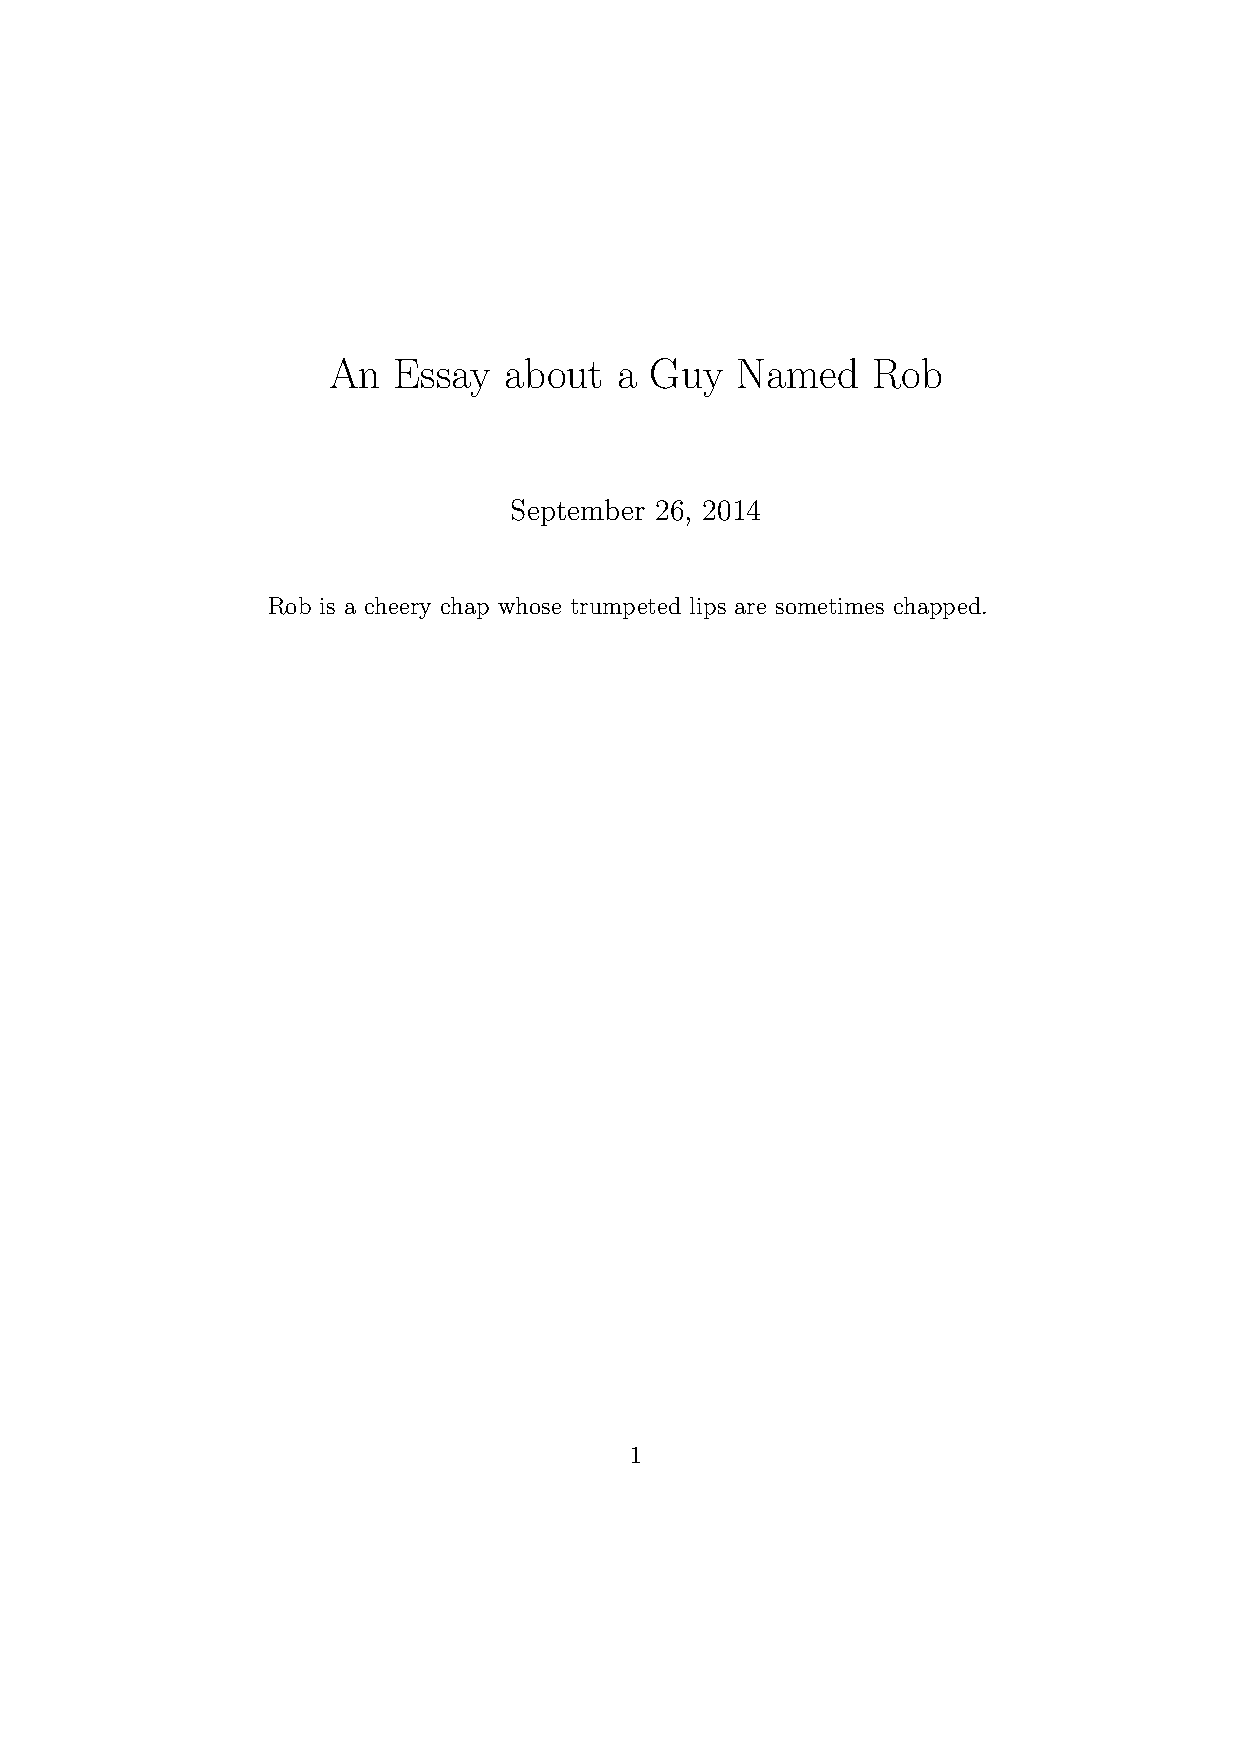
\includegraphics[scale=.4]{./chapters/02_basic/fakefile2}
  }
  \caption{Output from Example Input: \texttt{fakefile2.tex}}
\end{figure}

\marginpar{Go ahead and compile this document after you type it out.}

\clearpage

\section{Output File Structure}
\subsection*{Headings}

\begin{itemize}
\item \LaTeX~accepts the definition of a document hierarchy and displays
  headings appropriately. The \textit{article} class accepts the following
  headings whose order indicates how far down they are in the order:
  \texttt{\textbackslash part\{\}}, \texttt{\textbackslash section\{\}},
  \texttt{\textbackslash subsection\{\}}, \texttt{\textbackslash
    subsubsection\{\}}, \texttt{\textbackslash paragraph\{\}}, and
  \texttt{\textbackslash subparagraph\{\}}. If an ``\texttt{*}'' is placed after
  the name as in ``\texttt{\textbackslash part*\{\}}'' then the heading will not
  be numbered and will not be included in the table of contents, if it
  exists. Otherwise it will be numbered and included in the table of
  contents. The one mandatory argument is the text of the heading.

\item Any headings after the \verb=\appendix= command will be altered to reflect
  that they do not belong to the main body of the text and, rather, the
  appendix.

  \marginpar{Add a \texttt{section} and a \texttt{subsection*} heading to your
    document. Name them after your two favorite colors. Compile the document.}

\end{itemize}

\section{Environments}

\begin{itemize}
\item All of the content that will be displayed in your final document is
  contained in at least one environment. Environments are contexts which affect
  how the content is rendered and interpreted. Environments are indicated by the
  \verb=\begin{env}= and \verb=\end{env}= commands. We have already seen the
  \texttt{document} environment.

\item We will discuss various environments (and there are many) during the
  remainder of the week, but the basics are all the same. If you begin
  an environment, you must end it. When nesting environments, the most
  recently opened environment must be closed before an earlier
  environment can be closed.

\item The \texttt{enumerate} environment creates ordered lists. The
  \texttt{itemize} environment creates unordered lists. The
  \texttt{table} environment is used to encapsulate table-like content.

  \marginpar{At the end of your content begin and end a ``tiny''
    environment. Inside this environment type your favorite thing to shout. Use
    proper latex quotes (\textit{i.e.}\ ``\ldots '' and not
    "\ldots"). Compile the document.}

The insertion might look like

\begin{center}
  \begin{minipage}{.8\linewidth}
    \begin{framed}
\begin{verbatim}
\begin{tiny}
``Stellaaaaaaaaa!''
\end{tiny}
\end{verbatim}
    \end{framed}
  \end{minipage}
\end{center}

\end{itemize}

\section{Error Debugging}

You will, invariably, make errors. However, you'll probably never be
the first person to make any particular error. The four most common
errors are
\begin{enumerate}
\item you type a command incorrectly

\item you forget to \verb=\usepackage= the package that supplies a command which
  \LaTeX{} interprets as if you typed a command incorrectly

\item you don't \verb=\end{env}= what you \verb=\begin{env}= or you abuse the
  order of nested environments

\item you have un-balanced braces/parenthesis/brackets depending on
  what \LaTeX{} is looking for.

\end{enumerate}

Place the \texttt{tiny} environment inside a \texttt{center}
  environment. Now, change one of the \verb=\begin= commands to
    \verb=\benign=. Compile it. This is not benign! Look at the error
    message. Correct this mistake and swap the two \texttt{end}
    statements. Compile the document now. Look at the error message.


\section{Solving Problems and Getting Help}

\begin{itemize}
\item Don't panic.
\item Check the usual suspects.
\item Google a description of your problem in addition to ``latex
  ctan.'' Including ``latex'' without ``ctan'' is a bad, bad, bad,
  bad, bad idea!
\item Comment out potential sources of the problem until you
  identify it. Slowly add things back in until you have removed only
  the offending portion. Can this be fixed?

%% \item Consult one of the \LaTeX~ books in the star lab.

\item Consult one of the many great \LaTeX~sites out there.\footnote{Google
    either ``latex ctan wikibook'' or ``latex comprehensive symbol''. These two
    are great.}

\item Ask a friend!

%% \item Ask the star lab fellow!

\end{itemize}

%%% Local Variables:
%%% mode: latex
%%% TeX-master: "../../tutorial"
%%% End:


\clearpage
\pagebreak

\part{Creating Full Documents in \LaTeX}

\section{Starting Point}

\begin{itemize}

\item This section builds off of the previous one which introduced several
  \LaTeX{}~commands.

\item By the end of the last section we had working documents with environments
  and headings that were pleasing to the eye.

\item We will quickly create a very basic document to pick up where we
  left off.

\item Open your text editor and create a new \LaTeX{} file with a \texttt{*.tex}
  file extension wherever is most sensible to you.

\item Create a basic document with the following ``code'' and check that
  it compiles.

\lstinputlisting[caption=\texttt{fakefile3.tex}]{./chapters/03_full/fakefile3.tex}

\item Now, download the two dummy text files from
  \url{https://github.com/olmjo/LaTeX-Intro/tree/master/extra}. They are named
  \verb=loremipsum_short.txt= and \verb=loremipsum.txt=.

\item Place these two files in the same folder/directory as your new \LaTeX{}
  file.

\item As it stands, the document is quite bare. Modify the contents in the
  following way:
  \begin{itemize}

  \item Add \texttt{\textbackslash input\{./loremipsum\_short.txt\}}
    on a new line directly after \texttt{\textbackslash section\{Short
      Content\}}.

    That part of your \texttt{.tex} file should look like:

    \begin{lstlisting}
\section{Short Content}

\input{loremipsum_short}
     \end{lstlisting}


     As long as the downloaded file was placed in the
     appropriate place, you can safely ignore what this command does.

   \item Similarly, add \texttt{\textbackslash{}input\{./loremipsum.txt\}} on a new
     line directly after \texttt{\textbackslash{}section\{Long~Content\}}, as in

    \begin{lstlisting}
\section{Long Content}

\input{loremipsum}
     \end{lstlisting}

     As long as the downloaded file was placed in the appropriate place, you can
     safely ignore what this command does.
   \end{itemize}

 \item Compile this document again. You should have a document with a
   considerable amount of filler text in two of the sections.
\end{itemize}

\section{Fonts}

In \LaTeX{} we can make some very basic changes to the font in with ease. These
changes can be made with one of two approaches. The \textit{environment}
approach or the \textit{command} approach.

In the first, whatever font we change will be inside an environment. In the
second, whatever font we change will be the mandatory argument to a command.

\subsection*{Font Styles}
When displaying some text in \textbf{bold face} or \textsc{Small Caps}, we are
changing font styles.

The basic and most common changes are here:
\begin{small}
  \begin{center}
    \begin{tabular}{c c c}
      \hline
      Style               & Environment                                                                          & Command \\
      \hline
      normal/default      & \texttt{\textbackslash begin\{textnormal\} \ldots \textbackslash end\{textnormal\}}  & \texttt{\textbackslash textnormal\{\ldots \}}\\
      \textbf{bold}        & \texttt{\textbackslash begin\{bf\} \ldots \textbackslash end\{bf\}}  & \texttt{\textbackslash textbf\{\ldots \}}\\
      \textit{italics}     & \texttt{\textbackslash begin\{it\} \ldots \textbackslash end\{it\}}  & \texttt{\textbackslash textit\{\ldots \}}\\
      \textsc{SmallCaps}   & \texttt{\textbackslash begin\{sc\} \ldots \textbackslash end\{sc\}}  & \texttt{\textbackslash textsc\{\ldots \}}\\
      \underline{underline}&                                none  :-(                             & \texttt{\textbackslash underline\{\ldots \}}\\
      \textrm{Roman}       & \texttt{\textbackslash begin\{textrm\} \ldots \textbackslash end\{textrm\}}  & \texttt{\textbackslash textrm\{\ldots \}}\\
      \textsf{Sans Serif}  & \texttt{\textbackslash begin\{textsf\} \ldots \textbackslash end\{textsf\}}  & \texttt{\textbackslash textsf\{\ldots \}}\\
      \texttt{teletype}    & \texttt{\textbackslash begin\{tt\} \ldots \textbackslash end\{tt\}}  & \texttt{\textbackslash texttt\{\ldots \}}\\
      \hline
    \end{tabular}
  \end{center}
\end{small}

\begin{itemize}

\item Place the \texttt{\textbackslash{}input} command under the ``Short Content''
  section inside a font style environment of your choice. Compile the
  document.

  \begin{lstlisting}
\section{Short Content}

\begin{textsf}
  \input{loremipsum_short}
\end{textsf}
  \end{lstlisting}

\item Before this environment, but under the ``Short Content'' section type and
  complete the following sentence: ``If I had a boat, I'd \ldots''.

  \begin{lstlisting}
\section{Short Content}

If I had a boat, I'd go out on the ocean.
\begin{textsf}
  \input{loremipsum_short}
\end{textsf}
  \end{lstlisting}

\item Finally, change the style of the font for that sentence and only that
  sentence by using the command approach. This time, choose a different style
  from the environment change you made above.

  As an example,

  \begin{lstlisting}
\textbf{If I had a boat, \textit{I'd go out on the ocean}}.
  \end{lstlisting}

  gives

  \begin{center}
    \begin{minipage}{.5\linewidth}
      \begin{framed}
        \textbf{If I had a boat, \textit{I'd go out on the ocean}}.
      \end{framed}
    \end{minipage}
  \end{center}

\end{itemize}


\subsection*{Sizes}

The size the font can be modified in ways similar to how the font style was
changed.

\begin{small}
  \begin{center}
    \begin{tabular}{c c c}
      \hline
      Style               & Environment                                                                 & Command \\
      \hline
      \tiny{tiny}         & \texttt{\textbackslash begin\{tiny\} \ldots \textbackslash end\{tiny\}}      & \texttt{\textbackslash tiny\{\ldots\}}\\
      \scriptsize{scriptsize} & \texttt{\textbackslash begin\{scriptsize\} \ldots \textbackslash end\{scriptsize\}}      & \texttt{\textbackslash scriptsize\{\ldots\}}\\
      \footnotesize{footnotesize} & \texttt{\textbackslash begin\{footnotesize\} \ldots \textbackslash end\{footnotesize\}}      & \texttt{\textbackslash footnotesize\{\ldots\}}\\
      \small{small} & \texttt{\textbackslash begin\{small\} \ldots \textbackslash end\{small\}}      & \texttt{\textbackslash small\{\ldots\}}\\
      \normalsize{normalsize} & \texttt{\textbackslash begin\{normalsize\} \ldots \textbackslash end\{normalsize\}}      & \texttt{\textbackslash normalsize\{\ldots\}}\\
      \large{large} & \texttt{\textbackslash begin\{large\} \ldots \textbackslash end\{large\}}      & \texttt{\textbackslash large\{\ldots\}}\\
      \Large{Large} & \texttt{\textbackslash begin\{Large\} \ldots \textbackslash end\{Large\}}      & \texttt{\textbackslash Large\{\ldots\}}\\
      \LARGE{LARGE} & \texttt{\textbackslash begin\{LARGE\} \ldots \textbackslash end\{LARGE\}}      & \texttt{\textbackslash LARGE\{\ldots\}}\\
      \huge{huge} & \texttt{\textbackslash begin\{huge\} \ldots \textbackslash end\{huge\}}      & \texttt{\textbackslash huge\{\ldots\}}\\
      \Huge{Huge} & \texttt{\textbackslash begin\{Huge\} \ldots \textbackslash end\{Huge\}}      & \texttt{\textbackslash Huge\{\ldots\}}\\
      \hline
    \end{tabular}
  \end{center}
\end{small}

\begin{itemize}

\item Place the \texttt{\textbackslash input} command under the ``Long Content''
  section inside a font size environment of your choice, but choose a size that
  is smaller than the normal size.

    \begin{lstlisting}
\section{Long Content}

\begin{tiny}
  \input{loremipsum}
\end{tiny}
     \end{lstlisting}

  \item Compile your document.

\end{itemize}

\section{List Environments}

There are three main list environments that you will likely use:
\texttt{itemize}, \texttt{enumerate}, and \texttt{description}.

\begin{description}

\item[\texttt{itemize}] The \texttt{itemize} environment allows you to make
  bullet-ed lists without conveying any order. These can be nested to create any
  structure desired. However, complex nesting often results in user-mistakes.

\item[\texttt{enumerate}] The \texttt{enumerate} environment allows you to make
  numbered lists which convey a precise order. The numbering is
  automatic.\footnote{Like everything in \LaTeX{}, if it is important enough,
    you can override default. But, the guiding ethos of \LaTeX{} is that authors
    not spend long periods of time worrying about format rather than content.}
  These can be nested to create any structure desired and the ``numbering''
  system used at each level reflects how far in the tree the entry is.

\item[\texttt{description}] The \texttt{description} environment is slightly
  different. In fact, I am using it here to describe the different kinds of list
  environments. Instead of each entry being marked with an automatic bullet or
  number, the user must provide the ``term'' being described.
\end{description}

\begin{itemize}

\item For either \texttt{itemize} or \texttt{enumerate} your code
  looks like this, where ``\texttt{environment}'' is swapped out for
  the correct environment:

\begin{center}
  \begin{minipage}{.8\linewidth}
    \begin{framed}
\begin{verbatim}
\begin{environment} % itemize or enumerate
\item An item
\item Another item
\item Still more items!
\end{environment} % again, either itemize or enumerate
\end{verbatim}
    \end{framed}
  \end{minipage}
\end{center}

\item For the \texttt{description} environment your code is slightly
  different:

\begin{center}
  \begin{minipage}{.8\linewidth}
    \begin{framed}
\begin{verbatim}
\begin{description}
\item[An item] description 1
\item[Another item] description 2
\item[Still more items!] description 3
\end{verbatim}
    \end{framed}
  \end{minipage}
\end{center}


\item Create a list in the ``Some Book-keeping'' section. In this list you
  should have two items---two of your favorite books. The environment can be any
  of the three. If you are using the \texttt{description} environment include
  the author's name as the description if you know it. In this case, make sure
  the book title is in square brackets.
\end{itemize}

\section{Metadata: titles, dates, authors, abstracts}
\subsection*{\texttt{\textbackslash maketitle}}
\begin{itemize}
\item Although our content is already impressively long, the document
  is lacking all metadata. To address this we will formally introduce
  the \texttt{\textbackslash maketitle} command
\item In the preamble of the file (that is, before
  \texttt{\textbackslash begin\{document\}}, but after
  \texttt{\textbackslash documentclass}), enter the following code:

\begin{center}
  \begin{minipage}{.8\linewidth}
    \begin{framed}
\begin{verbatim}
\title{My First Opus}
\date{\today}
\author{Woodrow Wilson}
\end{verbatim}
    \end{framed}
  \end{minipage}
\end{center}


\item Compile the document. Notice that \textit{nothing} changes.

\item Now, add \texttt{\textbackslash{}maketitle} on a new line directly after
  \texttt{\textbackslash{}begin\{document\}} as in


\begin{center}
  \begin{minipage}{.8\linewidth}
    \begin{framed}
\begin{verbatim}

\title{My First Opus}
\date{\today}
\author{Woodrow Wilson}

% This is just a comment.
\begin{document}

\maketitle
\end{verbatim}
    \end{framed}
  \end{minipage}
\end{center}


\item Compile again.

\item Comment out the line with the \texttt{\textbackslash date}
  directive. Re-compile. What results from the following code?

\begin{center}
  \begin{minipage}{.8\linewidth}
    \begin{framed}
\begin{verbatim}

\title{My First Opus}
% \date{\today}
\author{Woodrow Wilson}

% This is just a comment.
\begin{document}

\maketitle
\end{verbatim}
    \end{framed}
  \end{minipage}
\end{center}


\item Uncomment that same line, delete the directive's single mandatory argument
  and compile. What happens from this code, instead?

\begin{center}
  \begin{minipage}{.8\linewidth}
    \begin{framed}
\begin{verbatim}

\title{My First Opus}
\date{}
\author{Woodrow Wilson}

% This is just a comment.
\begin{document}

\maketitle
\end{verbatim}
    \end{framed}
  \end{minipage}
\end{center}

\item In order to use the \texttt{\textbackslash{}maketitle} command, a title
  must be defined. The author and date, however are optional.

\end{itemize}

\subsection*{\texttt{\textbackslash{}thanks}}
\begin{itemize}
\item Woodrow Wilson is a humble man and acknowledges the contribution that
  non-Woodrow Wilson entities play in his success. To add this to the title we
  use \texttt{\textbackslash{}thanks}.

\item Include the following line at the end of ``Wilson'' within the author
  command as part of the mandatory argument: \texttt{\textbackslash{}thanks\{The
    author thanks Prospect House for having a sufficiently pretty garden.\}}

\begin{center}
  \begin{minipage}{.8\linewidth}
    \begin{framed}
\begin{verbatim}
\author{Woodrow Wilson\thanks{The author thanks
 Prospect House for having a sufficiently pretty garden.}
}
\end{verbatim}
    \end{framed}
  \end{minipage}
\end{center}

\item You can use \verb=\thanks= to include institution information or contact
  information, too. Or, you can use \verb=\footnote= which behaves the same way.

\end{itemize}


\subsection*{\texttt{titlepage}}

\begin{itemize}

\item Because this opus is so substantial, it can be overwhelming to
  assault the reader with content on the first page. In this case,
  we'd like to have just a title page.

\item Place the \verb=\maketitle= directive in an environment by the name of
  \texttt{titlepage}

\item Compile the document and see that there is now a title page separated from
  the content itself.

\end{itemize}

\subsection*{\texttt{abstract}}

\begin{itemize}

\item Even with a title, we might want to convey the content of our document in
  more detail.

\item In this case, we'd use an abstract.

\item After \verb=maketitle= but within the \verb=titlepage= environment, create
  a new environment (which is completely nested) called
  \texttt{abstract}. Within the \texttt{abstract} environment, write two
  sentences about what we have covered in this tutorial, so far. Include the
  word \LaTeX{}, properly typeset.

\item Compile the document.

\end{itemize}

\section{Fancy (and not Fancy) Headers}

\begin{itemize}

\item By default, the only content in the header or footer of our
  document is the page number.

\item We can change this by using a package called \texttt{fancyhdr}.

\item Tell \LaTeX{} to use this package. What is the command? Where
  does it go?

\item In the preamble, also include \verb=\pagestyle{plain}=.  Compile the
  document. What changes?

\item Now use \verb=\pagestyle{fancy}= instead. Compile the document. What
  changes?

\item You can change the contents of the headers and footers by using commands
  of the form \texttt{\textbackslash rfoot\{\}} for \texttt{r} (right),
  \texttt{l} (left), and \texttt{c} (center) ; and for \texttt{foot} (the
  footer) and \texttt{head} (the header).

\item Place the state or non-US country in which you were born somewhere in the
  footer. Compile the document.

\item Notice that the first page, the title page, has no header. Even when we
  use fancy headers and get the pretty content on that first inch of the page,
  any page with \verb=\maketitle= is unchanged, by default.

  We can change this by including \verb=\thispagestyle{fancy}= immediately after
  \verb=\maketitle=.
\end{itemize}


%%% Local Variables:
%%% mode: latex
%%% TeX-master: "../../tutorial"
%%% End:


\clearpage
\pagebreak

\part{Including Mathematics in \LaTeX{} Documents}

\section{Additional Packages}

\begin{itemize}

\item In order to avoid a lot of redundant and complicated code, it is
  helpful to load two particular packages each time you create a
  document with mathematics in it.

\item A bare-bones document requires only a \texttt{\textbackslash
    documentclass\{\}} line, followed by the \texttt{\textbackslash
    begin\{document\}} and \texttt{\textbackslash
    end\{document\}} lines.

\item We will now add \texttt{\textbackslash usepackage\{amsmath,
    amsthm, amssym, amsfonts\}} to the \textit{preamble} of the
  document. This tells \LaTeX{} to recognize certain commands defined
  in these packages.

\item We'll never use most of the functionality they add, but we'll
  often use some of it!

\item Create the following empty \LaTeX{} document in WinEdt in which
  we'll practice mathematical commands.

  \ovalbox{
    \begin{minipage}{\linewidth}
\begin{verbatim}
\documentclass{article}

\usepackages{amsmath, amsthm, amssymb, amsfonts}

% This is just a comment.

\begin{document}

\end{document}
\end{verbatim}
    \end{minipage}
  }

\end{itemize}

\section{Math Modes}

\begin{itemize}
  
\item In order to display mathematical content in \LaTeX{}, we will use a
  new set of commands that we wouldn't need for, say, writing a
  letter. However, \LaTeX{} doesn't allow you to issue these commands
  just anywhere. 

\item Rather, you need to be either in math mode or in a
  mathematical \textit{environment} where the math mode is implied.

\item There are two math modes which don't utilize special
  \textit{environments}: \textit{in-line} math and \textit{display
    math}.

\item These two are analogous to the way we include quotes in our own
  written work. \subparagraph{In-line} Sometimes the quotes are
  treated like any other text and printed in the same sized font
  without any special indentation. \subparagraph{Display} Sometimes
  the quotes begin on new lines, are indented, and quite distinct from
  the other text.

\item As a note, some commands and characters can only be entered in
  math mode. However, many, like the word ``computer'' can be entered
  in normal mode and math mode. Yet, if you think ``computer'' is
  different from ``$computer$'', then you must beware which mode you
  use.

\item After this section, it will be assumed that all math command
  sequence are typed in math mode. Otherwise, they will almost always
  fail. The math mode openings and closings are omitted.
  
\end{itemize}

\subsection*{In-line Math}
\begin{itemize}
\item The \textit{in-line} math mode is opened by typing a single
  dollar sign (\texttt{\$}) and then closed by typing a single dollar
  sign.
\item The content is placed in between the two \texttt{\$} symbols.
\item When we type \texttt{\$55/i = \textbackslash pi\^{}\{-0.3\}\$},
  we get $55/i = \pi^{-0.3}$. Any lines immediately following the
  in-line text are entirely unaffected, including this one. And
  this one, too.
\end{itemize}

\subsection*{Display Math}
\begin{itemize}
\item The \textit{display} math mode is opened by typing
  \texttt{\textbackslash [} and closed by typing
  \texttt{\textbackslash ]}. Another approach is to use double dollar
  signs as in the in-line mode (\texttt{\$\$ \ldots \$\$}). However,
  the square bracket approach is considered ``better''.

\item Again, the content to be displayed in the math mode is placed
  between the opening and closing key sequences.
\item Now, when we type \texttt{\textbackslash [55/i = \textbackslash
    pi\^{}\{-0.3\}\textbackslash ]}, we get
  \[
  55/i = \pi^{-0.3},
  \]
  which is the same as when we type \texttt{\$\$55/i = \textbackslash
    pi\^{}\{-0.3\}\$\$} and we get
  $$
  55/i = \pi^{-0.3}.
  $$
\item Clearly the appearance of the \textit{display} math is different
  from the \textit{in-line} math. However, sometimes the differences
  go beyond indentation and size. Both $\int_{0}^{\infty}
  \sum_{n=1}^{\infty} \frac{1}{n}~dx$ and 
\[
\int_{0}^{\infty} \sum_{n=1}^{\infty} \frac{1}{n}~dx
\]
have the same math mode code, but they are placed in the two different
modes. In this examples, the limits of integration are the most
obvious difference in how these expressions are rendered.
\end{itemize}

\section{Superscripts and Subscripts}
\begin{itemize}
\item To add a superscript to an expression use a hat,
  ``\texttt{\^{}}'', after the term with the exponent. So,
  \texttt{X\^{}3} gives $X^3$.

\item If your exponent has more than one character to be rendered in
  the case of $X^{3+y}$, then we must surround the entire exponent in
  \textit{curly braces} (\texttt{\{ \}}). For this previous expression
  we'd type \texttt{X\^{}\{3+y\}}. In this sense, the
  \textit{curly braces} group terms. When in doubt, use curly braces
  to set the scope of your exponent. Had we omitted the curly braces,
  we'd see $X^3+y$ which is quite different.

\item The principle for subscripting is identical, but we use the
  underscore, ``\texttt{\_}'', instead. Typing
  \texttt{X\_{}\{3+y\}} gives $X_{3 + y}$.

\item Super-- and subscripting can be recursive. However, one must be
  very careful with braces in this case. We can typeset $e^{x_{i}}$
  with \texttt{e\^{}\{x\_\{i\}\}}. Now, the braces around the
  \texttt{i} term are optional. Remove them, what happens to the
  rendering? Remove the braces around the $x_i$ term. Compile the
  document. What happens to the rendering?

\item Both superscripts and subscripts can be used simultaneously. In
  Social Choice, we often care about the median voter's preference,
  denoted $x_i^m$. This can be achieved with either
  \texttt{x\_i\^{}m} or \texttt{x\_\{i\}\^{}\{m\}}. The latter
  is more typing, but forces you to be explicit about the scope which
  tends to reduce the number of errors.

\end{itemize}

\section{Operators}

\begin{multicols}{3}
\begin{itemize}
\item[$+$] \texttt{+}
\item[$=$] \texttt{=}
\item[$-$] \texttt{-}
\item[$/$] \texttt{/}
\item[$<$] \texttt{<}
\item[$>$] \texttt{>}
\item[$\leq$] \texttt{\textbackslash leq}
\item[$\geq $] \texttt{\textbackslash geq}
\item[$\vee$] \texttt{\textbackslash vee}
\item[$\wedge$] \texttt{\textbackslash wedge}
\item[$\bigvee$] \texttt{\textbackslash bigvee}
\item[$\bigwedge$] \texttt{\textbackslash bigwedge}
\item[$\cup$] \texttt{\textbackslash cup}
\item[$\cap$] \texttt{\textbackslash cap}
\item[$\bigcup$] \texttt{\textbackslash bigcup}
\item[$\bigcap$] \texttt{\textbackslash bigcap}
\item[$\forall$] \texttt{\textbackslash forall}
\item[$\exists$] \texttt{\textbackslash exists}
\item[$\subset$] \texttt{\textbackslash subset}
\item[$\subseteq$] \texttt{\textbackslash subseteq}
\item[$\subsetneq$] \texttt{\textbackslash subsetneq}
\item[$\supset$] \texttt{\textbackslash supset}
\item[$\supseteq$] \texttt{\textbackslash supseteq}
\item[$\supsetneq$] \texttt{\textbackslash supsetneq}
\item[$\int$] \texttt{\textbackslash int}
\item[$\sum$] \texttt{\textbackslash sum}
\item[$\prod$] \texttt{\textbackslash prod}
\item[$\partial$] \texttt{\textbackslash partial}
\item[$\sim$] \texttt{\textbackslash sim}
\item[$\approx$] \texttt{\textbackslash approx}
\item[$\Leftrightarrow$] \texttt{\textbackslash Leftrightarrow}
\item[$\leftrightarrow$] \texttt{\textbackslash leftrightarrow}
\item[$\Leftarrow$] \texttt{\textbackslash Leftarrow}
\item[$\leftarrow$] \texttt{\textbackslash leftrightarrow}
\item[$\Rightarrow$] \texttt{\textbackslash Rightarrow}
\item[$\rightarrow$] \texttt{\textbackslash rightarrow}
\item[$\not ~$] \texttt{\textbackslash not}
\item[$\neg$] \texttt{\textbackslash neg}
\item[$\div$] \texttt{\textbackslash div}
\item[$\infty$] \texttt{\textbackslash infty}
\item[$\emptyset$] \texttt{\textbackslash emptyset}
\item[$\in$] \texttt{\textbackslash in}
\end{itemize}
\end{multicols}

\section{Greek Letters}

\begin{itemize}
\item Greek letters are uncomfortably common in the work we do, so you
  will get used to including them in your documents.

\item Although there are neither $\zeta$ nor $\chi$ keys on your
  keyboard, we can include these symbols in the math environment in a
  very intuitive way. Type \texttt{\textbackslash name-of-letter}
  or \texttt{\textbackslash Name-of-letter} for the lower-case and
  upper-case version of the Greek letter.

\item So, \texttt{\textbackslash delta} and \texttt{\textbackslash
    Delta} give $\delta$ and $\Delta$, respectively.

\item Not every letter has a special upper-case version
  provided. Although \texttt{\textbackslash beta} gives $\beta$
  \texttt{\textbackslash Beta} is undefined.

\item Not every letter has a special character, regardless of
  case. For example, the Greek omicron is just like the Roman `o', so
  \texttt{o} gives $o$ which will be sufficient.

\item With Greek letters a particular issue arises often, although it
  isn't specific to Greek letters. \LaTeX{} commands do not need a
  leading space before the \texttt{\textbackslash}. Yet, they do need
  a trailing space so that \LaTeX{} knows the name of the command is
  over. So, \texttt{X\textbackslash beta} ($X\beta$) is rendered
  identically to \texttt{X~\textbackslash beta} ($X \beta$)
  because \LaTeX{} has its own way of interpreting
  whitespace. However, \texttt{X\textbackslash beta + \textbackslash
    epsilon} ($X\beta + \epsilon$) works whereas
  \texttt{X~\textbackslash beta+ \textbackslash epsilon} will not
  because \texttt{\textbackslash beta+} is an undefined control
  sequence (i.e. we just made up that command).

\end{itemize}
\section{Other Letter-y Things}

Sometimes we need to present change the presentation of standard
letters or symbols in math mode. Here are several common examples. The
way these work is that whatever symbols are to have their face changed
are passed to these commands as arguments. Notice how the ``math''
faces remove white space

\begin{tabular}{c c c c}
  \hline \hline
  Modification & Command & Example & Common Uses\\
  \hline
  Normal Math Face & ---& $ABC XY$ & most maths\\
  Roman Face & \texttt{\textbackslash textrm\{\}} &  $\textrm{ABC XY}$& text within equation\\
  Bold Math Face & \texttt{\textbackslash mathbf\{\}} &  $\mathbf{ABC XY}$ & vectors and matrices\\
  Blackboard Math & \texttt{\textbackslash mathbb\{\}} &  $\mathbb{ABC XY}$ & special sets of numbers\\
  Calligraphic Math & \texttt{\textbackslash mathcal\{\}} & $\mathcal{ABC XY}$& arbitrary sets\\
  \hline \hline
\end{tabular}

\section{Special Text-like Mathematical Expressions}

Certain functions, operators, and constructs pop up in math frequently
which are basically abbreviates for words. The cosine function---as in
$\cos(\pi)=1$---and the limit of an expression---as in $\lim_{x
  \rightarrow \infty} \frac{1}{x}$---are two such examples. If we just
typed \texttt{\$cos\$} ($cos$) or \texttt{\$lim\$} ($lim$) we get
results quite different. An incomplete list of the expressions for
which the control sequences are defined is below.

\begin{multicols}{4}
\begin{itemize}
\item[$\det$] \texttt{\textbackslash det}
\item[$\lim$] \texttt{\textbackslash lim}
\item[$\max$] \texttt{\textbackslash max}
\item[$\min$] \texttt{\textbackslash min}
\item[$\inf$] \texttt{\textbackslash inf}
\item[$\sup$] \texttt{\textbackslash sup}
\item[$\cos$] \texttt{\textbackslash cos}
\item[$\sin$] \texttt{\textbackslash sin}
\item[$\tan$] \texttt{\textbackslash tan}
\item[$\exp$] \texttt{\textbackslash exp}
\item[$\Pr$] \texttt{\textbackslash Pr}
\item[$\arg$] \texttt{\textbackslash arg}
\end{itemize}
\end{multicols}

\section{Delimiters}
Many times, we need to express groupings through the use of
delimiters. For example, $(100 - 100)^{100}$ is quite different than
$100 - 100^{100}$. For parentheses we can just enter \texttt{(x)}. For
curly braces we enter \texttt{\{x\}}. And, lastly, for square brackets
we use \texttt{[x]}. These produce $(x)$, $\{x\}$, and $[x]$,
respectively. In longer expressions, though, the results can look
funny.
In
\[
[\sum_{x=1}^{3} \{ (\int_{0}^{x} (e^{y}~dy))\}],
\]
the size of the delimiters is off. However, in
\[
\left[\sum_{x=1}^{3} \left\{ \left(\int_{0}^{x} (e^{y}~dy)\right)\right\}\right],
\]
the problems seem to be gone. If we type \texttt{\textbackslash
  left(}, \texttt{\textbackslash left\textbackslash\{}, or
\texttt{\textbackslash left[} and close the expression off with the
approprate \texttt{\textbackslash right)}, \texttt{\textbackslash
  right\textbackslash\}}, or \texttt{\textbackslash right]}, the sizes
are determined by the size of the internal expression as opposed to
being constant.
\section{Accents}

Often times we need to modify slightly a character it denote that the
construct has slightly changed. For example, we want
\begin{itemize}
\item not the true parameter $\beta$ but the estimate $\hat{\beta}$,
\item not the random variable $y$, but the sample mean $\bar{y}$, or
\item not the singleton $x$, but a vector $\vec{x}$.
\end{itemize}

A partial list of these accents is below.
\begin{multicols}{3}
\begin{itemize}
\item[$\acute{a}$] \texttt{\textbackslash acute\{a\}}
\item[$\bar{b}$] \texttt{\textbackslash bar\{b\}}
\item[$\breve{c}$] \texttt{\textbackslash breve\{c\}}
\item[$\check{d}$] \texttt{\textbackslash check\{d\}}
\item[$\dot{e}$] \texttt{\textbackslash dot\{e\}}
\item[$\ddot{f}$] \texttt{\textbackslash ddot\{f\}}
\item[$\grave{g}$] \texttt{\textbackslash grave\{g\}}
\item[$\hat{h}$] \texttt{\textbackslash hat\{h\}}
\item[$\tilde{\imath}$] \texttt{\textbackslash tilde\{\textbackslash imath\}}
\item[$\vec{\jmath}$] \texttt{\textbackslash vec\{\textbackslash jmath\}}
\item[$\widehat{xyz}$] \texttt{\textbackslash widehat\{\textbackslash xyz\}}
\item[$\widetilde{xyz}$] \texttt{\textbackslash widetilde\{\textbackslash xyz\}}

\end{itemize}
\end{multicols}

\section{Assignment!}

\subsection*{Questions}
Write \LaTeX{} code for the following expressions. Confirm that your
compiled document matches these.
\begin{enumerate}
\item
\[
\neg\left(\left(T \vee F\right) \wedge F\right) \vee \left( T \right)
\]

\item 
\[
e^{ix} = \cos x + i \sin x
\]

\item
\[
y_i = \beta_0 + \beta_1 x_i + \beta_2 x_i^2 + \epsilon_i
\]

\item
\[
\left(\sum_{x=1}^{\infty} (1/x) \right) - \left(\sum_{x=1}^{\infty}
  (1/x)^2 \right)
\]
\end{enumerate}

\subsection*{Answers}

\begin{enumerate}

\item ~\\
  \begin{turn}{180}
  \ovalbox{
    \begin{minipage}{\linewidth}
\begin{verbatim}

\[
\neg\left(\left(T \vee F\right) 
\wedge F\right) \vee \left( T \right)
\]

\end{verbatim}
    \end{minipage}
  }
\end{turn}

\item ~\\
  \begin{turn}{180}
  \ovalbox{
    \begin{minipage}{\linewidth}
\begin{verbatim}

\[
e^{ix} = \cos x + i \sin x
\]

\end{verbatim}
    \end{minipage}
  }
\end{turn}

\item ~\\
  \begin{turn}{180}
  \ovalbox{
    \begin{minipage}{\linewidth}
\begin{verbatim}

\[
y_i = \beta_0 + \beta_1 x_i + 
\beta_2 x_i^2 + \epsilon_i
\]

\end{verbatim}
    \end{minipage}
  }
\end{turn}

\item ~\\
  \begin{turn}{180}
  \ovalbox{
    \begin{minipage}{\linewidth}
\begin{verbatim}

\[
\left(\sum_{x=1}^{\infty} (1/x) \right) - 
\left(\sum_{x=1}^{\infty}
  (1/x)^2 \right)
\]

\end{verbatim}
    \end{minipage}
  }
\end{turn}

\end{enumerate}


%%%%%%%%%%%%%%%%%%%%%%%%%%%%%%%%%%%%%%%%%%%%%%%%%%%%%%%%%%%%%%%%%%%%%%%%%%%%%%% 
%%%%%%%%%%%%%%%%%%%%%%%%%%%%%%%%%%%%%%%%%%%%%%%%%%%%%%%%%%%%%%%%%%%%%%%%%%%%%%% 
%%%%%%%%%%%%%%%%%%%%%%%%%%%%%%%%%%%%%%%%%%%%%%%%%%%%%%%%%%%%%%%%%%%%%%%%%%%%%%% 

\clearpage
\pagebreak

%% \part{\LaTeX{} Miscellany}

\section{Tables}
\begin{itemize}
\item We can create tabular content in a \LaTeX{} document either within
  a float environment or not. We will describe what a float is in a moment.
  
\item Either way, tabular content like the following is created with
  the \texttt{tabular} environment.

  \begin{center}
    \begin{tabular}{c c c} 
      \hline 
      \hline
      Student & Alma Mater & Favorite Color \\
      \hline
      Tyson Chatagnier & Texas A\&M & Denim \\
      Jonathan Klingler & Notre Dame & Green \\
      Gary Hollibaugh & UCSD & Orange and Aquamarine \\
      Jonathan Olmsted & UDel & French Blue \\
      Peter Haschke & UNC-Asheville & Titian Red \\
      Lukas Pfaff & Iowa State University & Cornflower blue\footnote{This is not necessarily true, it is, however, just a corn joke!'}\\
      \hline
      \hline
    \end{tabular}
  \end{center}

\item The \texttt{tabular} environment takes a mandatory argument that
  is enclosed in curly braces. In the case of the above table where
  each column is center justified, we'd use
  \verb! \begin{tabular}{c c c} \end{tabular}!. If we wanted the
  columns to be right-justified or left-justified we could use
  \texttt{r} or \texttt{l}.
  \item If we wanted to add a vertical line on either the left or right or in-between two columns we'd use the  argument \verb!{| c | c | c |}!.
  \item Horizontal lines are given by \verb!\hline!.
  \item Tab breaks are caused by \verb!&! and line breaks by \verb!\\!.
  \item The full code for the above table is:\\
    \ovalbox{
      \begin{minipage}{\linewidth}
\begin{verbatim}

  \begin{center}
    \begin{tabular}{c c c} 
      \hline 
      \hline
      Student & Alma Mater & Favorite Color \\
      \hline
      Tyson Chatagnier & Texas A\&M & Denim \\
      Jonathan Klingler & Notre Dame & Green \\
      Gary Hollibaugh & UCSD & Orange and Aquamarine \\
      Jonathan Olmsted & UDel & French Blue \\
      Peter Haschke & UNC-Asheville & Titian Red \\
      Lukas Pfaff & Iowa State University & Cornflower blue
      \footnote{This is not necessarily true, it is, 
        however, just a corn joke!'}\\
      \hline
      \hline
    \end{tabular}
  \end{center}

\end{verbatim}
    \end{minipage}
  }

\item The line breaks and whitespace in the above code are poorly
  selected, but this results from the need to fit the code in such a
  small block. Usually, the code for \LaTeX{} tables can be several
  times wider than anything else in your \LaTeX{} document.

\item There are much more complex environments than 
  \texttt{tabular} that you will have to use once your 
  tabular content grows. They are similar, but have 
  their own documentation to help you through. 
  \end{itemize}
  
\section{Pictures}
\begin{itemize}
\item \LaTeX{} has the ability to draw arbitrary types of objects and
  schematics within a \LaTeX{} document in a native language. However,
  this is seldom used and probably less advantageous than including
  external files.

\item Download \texttt{Image1.pdf} and \texttt{Image2.png} from
  \url{www.rochester.edu/college/gradstudents/jolmsted/}

\item In your preamble, add the \texttt{graphicx} package (i.e.\
  \verb!\usepackage{graphicx}!)

\item Where you'd like the picture to show up, type
  \verb!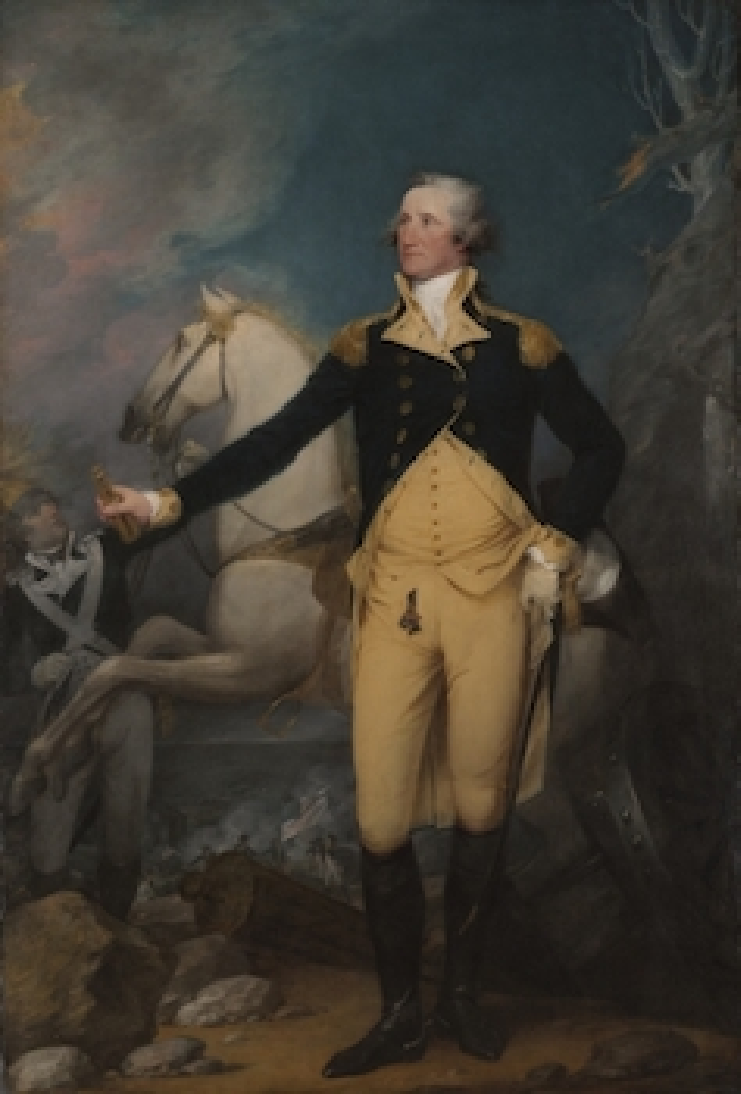
\includegraphics{./Image1}! without a file extension and be
  sure to use the appropriate path to the image file, relative to the
  \LaTeX{} document. The file extension is not necessary.
\item The \verb!scale! optional argument is useful to change
  dimensions on the fly without distorting the aspect ratio.
\item Try the following code in a \LaTeX{} document environment:
  
  \ovalbox{
    \begin{minipage}{\linewidth}
\begin{verbatim}

  \begin{center}
    \fbox{
      \fbox{
        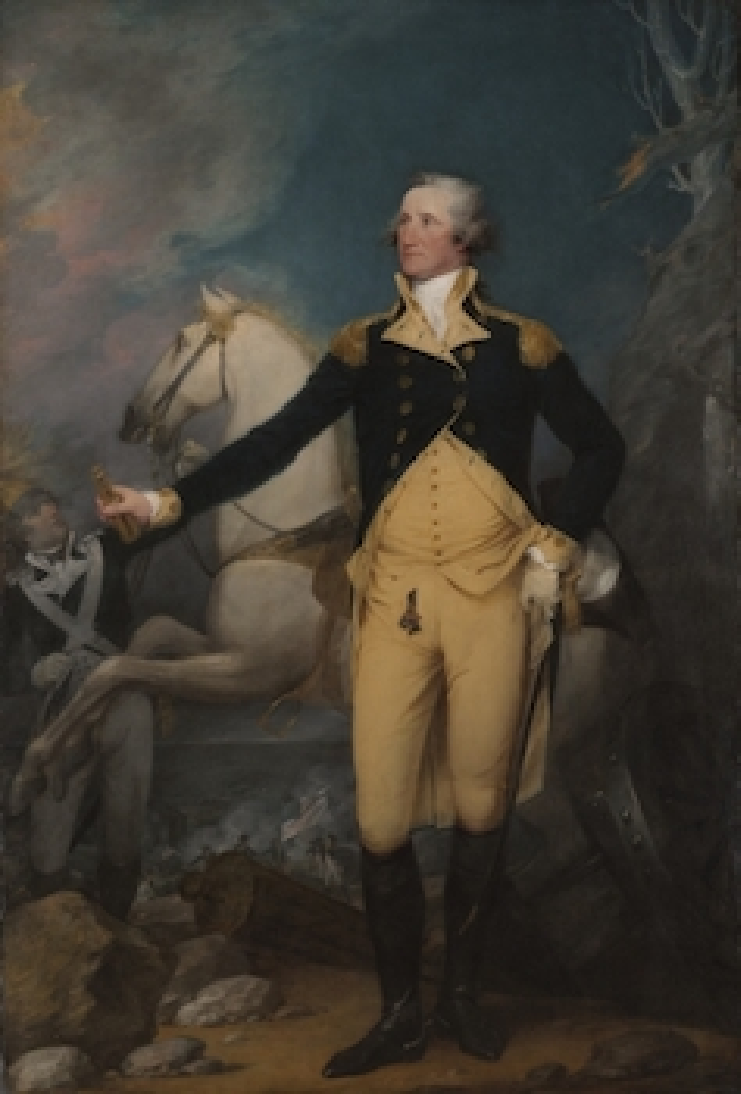
\includegraphics[scale=.25]{./Image1}
      }
      \fbox{
        \includegraphics[width=3in, 
        height=1in, 
        angle=90]{./Image2}
      }
    }
  \end{center}

\end{verbatim}
    \end{minipage}
  }

\item The result is something like 
  \begin{center}
    \fbox{
      \fbox{
        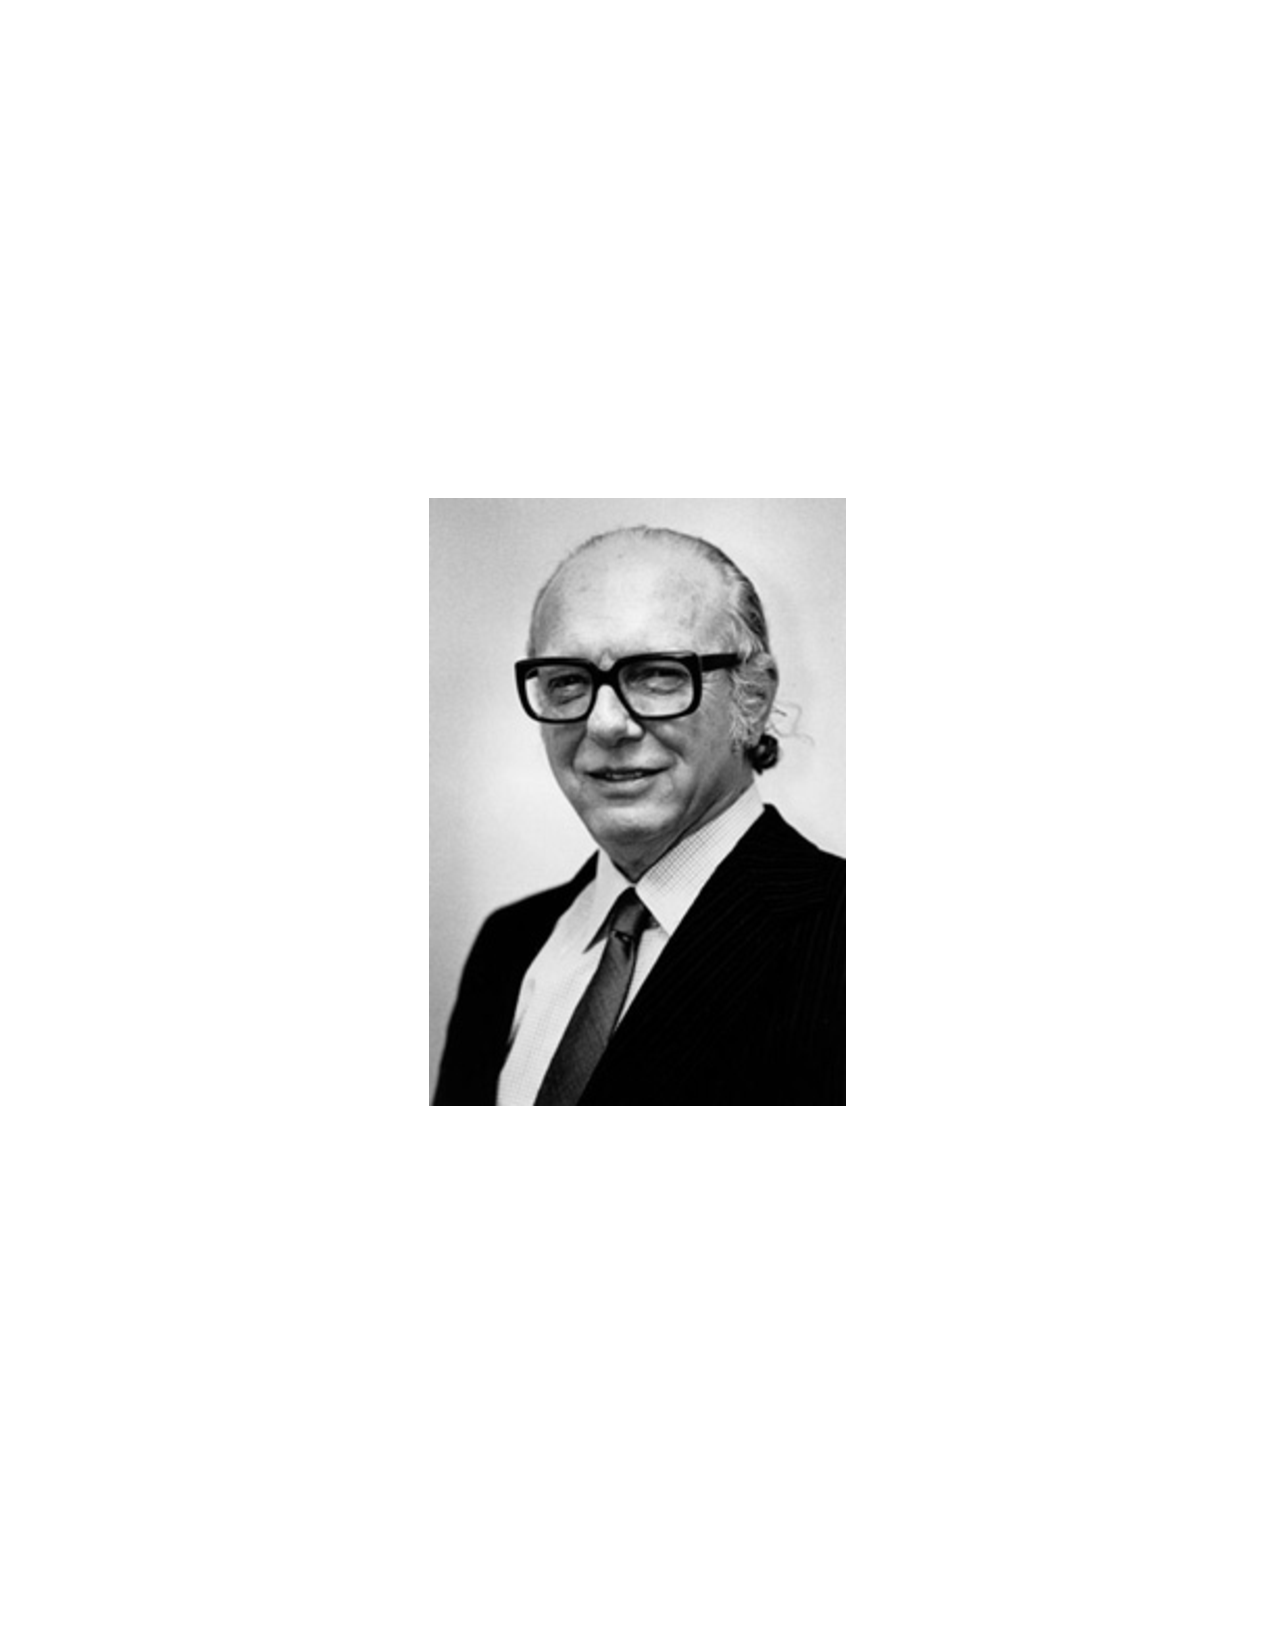
\includegraphics[scale=.25]{../5_Misc/Image1}
      }
      \fbox{
        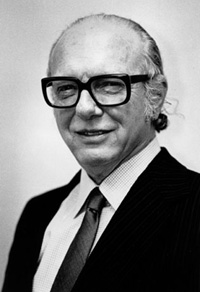
\includegraphics[width=3in, 
        height=1in, 
        angle=90]{../5_Misc/Image2}
      }
    }
  \end{center}

\item Notice that we didn't have to specify the file extension. Notice
  the order in which the \texttt{angle} and then
  \texttt{height}/\texttt{width} arguments are applied. What does
  \verb!\fbox{}! do?
    

\end{itemize}

\section{Floats}
\begin{itemize}
\item Although we can create tables with the \texttt{tabular}
  environment and we use \verb!\includegraphics{}! to insert external
  image files, these commands are seldom placed inside a document
  without entering them in a special environment.
\item Typically, these kinds of content are placed in \textit{floats}
  which act like containers for tables and figures. \LaTeX{},
  according to a set of rules, figures where these containers should
  be placed which depends on the content before the float, the content
  after the float, and the \LaTeX{} code within the float.

\item If nothing else, the big adjustment required by users placing
  content in floats is realizing that the placement of a table or
  figure is up to \LaTeX{} and
  ``jury-rigging''/''jimmy-rigging''/''jerry-rigging'' the placement
  is ill-advised.

\item The float for tables is
  \verb!\begin{table}[htpb] \end{table}!. The optional \verb![thpb]!
  argument provides \LaTeX with some instructions on where to place
  the table.

\item The float environment for figures is
  \verb!\begin{figure}[htpb] \end{figure}!. Notice, again, the
  optional argument.

\item In actuality, there need not be anything inside these float
  environments, or it could easily be regular \LaTeX{} markup.

\item \verb!\caption{}!, placed somewhere in the float, allows a title
  of the content to be placed and automatically numbered.

\item \verb!\label{}!, placed immediately after the \verb!\caption{}!
  command gives an identified to the object by which it can be
  referred for directing readers to Figure 1 or Table 4 without
  hard-coding the float order.

\item Try: \\
  \ovalbox{
    \begin{minipage}{\linewidth}
\begin{verbatim}
\begin{figure}
  \begin{center}
    \fbox{
      \includegraphics[width=3in, 
      height=1in, 
      angle=120]{./Image2}
    }
    \caption{A Hero of a Man} \label{f:Riker}
  \end{center}
\end{figure}
\end{verbatim}
    \end{minipage}
  }

\item Now, see Figure \ref{f:Riker} on page \pageref{f:Riker} to view
  the output. We were able to reference the figure number
  automatically using \verb!\ref{f:Riker}! which matches our
  \verb!\label!. We reference the page number automatically with \verb!\pageref{}!.
  \\

\begin{figure}
  \begin{center}
    \fbox{
      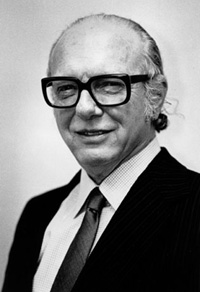
\includegraphics[width=3in, 
      height=1in, 
      angle=120]{../5_Misc/Image2}
    }
    \caption{A Hero of a Man} \label{f:Riker}
  \end{center}
\end{figure}

\end{itemize}

\section*{More Math Environments}
\begin{itemize} 
\item There are a number of math environments that become useful when
  one is typesetting mathematical notation beyond very basic
  experessions.
\item As in a previous tutorial, add
  \verb!\usepackage{amsmath, amsthm, amssymb, amsfonts}! to the
  preamble if not already there.
\end{itemize}

\subsection*{Fraction}
There are instances where $3/4$ would look better as $\frac{3}{4}$ and
this works equally well for longer expressions $$
\frac{\tan\left(\cos\left(\sin (X) \right)\right)}{\int_{\mathbb{R}}
  f(x) ~ dx}.$$ It is the command \verb!\frac{}{}! which provides
this. The numerator is the first argument and the denominator is the
second.
\subsection*{Equation}
The equation environment is a very common way to typeset equations
when reference numbers are being used. So, for example,
\verb!\begin{equation} 4=x^2 \end{equation}! gives 
\begin{equation}
  4=x^2.
\end{equation}
Now, it is not necessary to place the equation environment in a math
mode. In this sense, the math mode is implied. There is also a variant
such that \verb!\begin{equation*} 4=x^2 \end{equation*}! suppresses
the equation numbering,
\begin{equation*} 
  4=x^2.
\end{equation*}
Equation numbers can be labeled and referenced as was done in the
figure environment. This is a single equation environment and if you
try to enter line breaks such that you could force another line, it
will fail. In that case, I find the \texttt{align} approach being the
easiest because it is flexible.

\subsection*{Align}
The \texttt{align} environment allows you to enter multiple lines and
include alignment stops. There is a un-numbered version,
\texttt{align*}, too. The code

\ovalbox{
    \begin{minipage}{\linewidth}
\begin{verbatim}
\begin{align}
   \sum_{x=1}^{4} \frac{1}{x} &
   &= \frac{1}{1} + \frac{1}{2}  + \frac{1}{3} + \frac{1}{4} & \\
   &= \frac{25}{12} &\\
   & &>2   
\end{align}
\end{verbatim}
    \end{minipage}
  }
produces a three line \texttt{align} environment.
\begin{align}
   \sum_{x=1}^{4} \frac{1}{x}
   &= \frac{1}{1} + \frac{1}{2}  + \frac{1}{3} + \frac{1}{4} \\
   &= \frac{25}{12} \\
   &>2   
\end{align}
Notice that the numbering is cumulative. The use of \verb!\label{}!
and \verb!ref{}! works identically here.


\subsection*{Array}
The \texttt{array} environment provides a unified way of representing
vectors and matrices. The environment begins in the standard
\verb!\begin{array}{cc} \end{array}! way, but the mandatory
\verb!{cc}! argument specifies there are two center-justified
columns. Changes to this argument proceed identically to the argument
in the creation of tables. On important point is that the array
environment does not create its own math mode environment, so we must
put it inside one when we use it. We get \[ \left[\begin{array}{cc} 1 & 0 \\
    0 & 1\end{array}\right], \] the two dimensional identity matrix
from \\
\ovalbox{
    \begin{minipage}{\linewidth}
\begin{verbatim}
\[
 \left[
\begin{array}{cc} 
  1 & 0 \\
  0 & 1
\end{array}
\right],
\]
\end{verbatim}
    \end{minipage}
  } \\ Notice the comma in the source code. It must be in the display
  math environment so that it is placed adjacent to the matrix and not
  in the text. By changing the number of rows, columns, and the
  delimiters, most matrix-like objects can be represented with this
  environment.

\subsection*{Cases}

The \texttt{cases} environment is both extremely useful, but quite
narrow in application. Although it is designed to be used only to
represent piece-wise functions, it is a marked improvement over the
alternative which would be to ``hack'' the \texttt{array}
environment. Like the \texttt{array} environment, though,
\texttt{cases} must be used within math mode. So, 

\[
\mathbf{1}_{\mathcal{X}}(x) = 
\begin{cases}
  1, & x \in \mathcal{X} \\
  0, & \textrm{otherwise}
\end{cases}
\]
is the result of the code

\ovalbox{
    \begin{minipage}{\linewidth}
\begin{verbatim}
\[
\mathbf{1}_{\mathcal{X}}(x) = 
\begin{cases}
  1, & x \in \mathcal{X} \\
  0, & \textrm{otherwise}
\end{cases}.
\]
\end{verbatim}
    \end{minipage}
  } Notice how I use whitespace and line breaks to organize the code
  although \LaTeX{} won't interpret it.

\section{Words of Wisdom}

\begin{itemize}
\item It is considered good practice to keep text file contents within
  the first 80 characters. This may seem weird or hard, but this,
  along with use of the \texttt{\%} and comments will make the input
      file more human-readable.
    \item As you learn \LaTeX{} don't worry about trying to make
      \LaTeX{} look a certain way. Tell \LaTeX{} about your content
      and its structure. Let \LaTeX{} worry about the details of
      appearance.
    \item Google is your friend.

    \item Comment out error-laden parts of code. Add things back in
      one at a time until you've identified the source of your
      syntactical mistakes.

    \item Let WinEdt help you. It highlights the source file according
      to rules. If the rules are broken, the highlighting will appear
      other it should and this is a visual cue that something is
      wrong.

    \item Because \LaTeX{} seldom interprets whitespace in too
      generous a way, use it as an organizational tool.
\end{itemize}

% \end{document}


%%%%%%%%%%%%%%%%%%%%%%%%%%%%%%%%%%%%%%%%%%%%%%%%%%%%%%%%%%%%%%%%%%%%%%%%%%%%%%% 
%%%%%%%%%%%%%%%%%%%%%%%%%%%%%%%%%%%%%%%%%%%%%%%%%%%%%%%%%%%%%%%%%%%%%%%%%%%%%%% 
%%%%%%%%%%%%%%%%%%%%%%%%%%%%%%%%%%%%%%%%%%%%%%%%%%%%%%%%%%%%%%%%%%%%%%%%%%%%%%% 



\clearpage



%% \bibliographystyle{}
%% \bibliography{}

\end{document}

%%%%%%%%%%%%%%%%%%%%%%%%%%%%%%%%%%%%%%%%%%%%%%%%%%%%%%%%%%%%%%%%%%%%%%%%%%%%%%%
%%%%%%%%%%%%%%%%%%%%%%%%%%%%%%%%%%%%%%%%%%%%%%%%%%%%%%%%%%%%%%%%%%%%%%%%%%%%%%%
%%%%%%%%%%%%%%%%%%%%%%%%%%%%%%%%%%%%%%%%%%%%%%%%%%%%%%%%%%%%%%%%%%%%%%%%%%%%%%%

%%% Local Variables:
%%% mode: latex
%%% TeX-master: t
%%% End:
